\documentclass[12pt,letterpaper]{article}

%\usepackage{fixltx2e}
\usepackage{textcomp}
\usepackage{fullpage}
\usepackage{amsfonts}
\usepackage{verbatim}
\usepackage[english]{babel}
\usepackage{pifont}
\usepackage{color}
\usepackage{setspace}
\usepackage{lscape}
\usepackage{indentfirst}
\usepackage[normalem]{ulem}
\usepackage{booktabs}
%\usepackage{nag}
%\usepackage{natbib}
%\usepackage{bibtex}
\usepackage{float}
\usepackage{latexsym}
%\usepackage{hyperref} 
\usepackage{url}
%\usepackage{html}
\usepackage{hyperref}
\usepackage{epsfig}
\usepackage{graphicx}
\usepackage{amssymb}
\usepackage{amsmath}
\usepackage{bm}
\usepackage{array}
%\usepackage{mhchem}
\usepackage[version=4]{mhchem}
\usepackage{ifthen}
\usepackage{caption}
\usepackage{hyperref}
%\usepackage{xcolor}
\usepackage{amsthm}
\usepackage{amstext}
\usepackage{enumerate}
\usepackage{csquotes}
\usepackage{setspace}
\usepackage{longtable}
\usepackage{lscape}
\usepackage{algorithmic}

% Add and remove packages as necessary for your manuscript.
%\RequirePackage{lineno}

%\setlength{\extrarowheight}{20pt}
\linespread{1.66}
% All text should be double-spaced
% with occasional exceptions for tables. 
\raggedright
\setlength{\parindent}{0.5in}

\setcounter{secnumdepth}{0}
% Our sections are not numbered and our papers do not have
% Tables of Contents. We don't 
% present a list of figures or list of tables, either.

% Any common font is fine.
% (A common sans-serif font should be used on figures, but figures should be
% separate from the LaTeX document.)
%\pagestyle{empty}

\renewcommand{\section}[1]{%
\bigskip
\begin{center}
\begin{Large}
\normalfont\scshape #1
\medskip
\end{Large}
\end{center}}

%\renewcommand{\subsection}[1]{%
%\bigskip
%\begin{center}
%\begin{large}
%\normalfont\itshape #1
%\end{large}
%\end{center}}

%\renewcommand{\subsubsection}[1]{%
%\vspace{2ex}
%\noindent
%\textit{#1.}---}
\def\doubleq#1{``#1''}
\def\singleq#1{`#1'}

%\renewcommand{\tableofcontents}{}

%\usepackage{natbib}
%\bibpunct{(}{)}{;}{a}{}{,}  % this is a citation format command for natbib

%%% NUMBERED BIB
%\usepackage[round,numbers,sort&compress]{natbib}
%\renewcommand{\bibnumfmt}[1]{#1.}
%%% NUMBERED BIB SUPERSCRIPT
\usepackage[super,comma,sort&compress]{natbib} 
\renewcommand{\bibnumfmt}[1]{#1.}

\newcommand{\T}{{\theta}} 
\newcommand{\TP}{{\theta^{\prime}}}
\newcommand{\UB}{{\mathbf{u}}}

\newcommand{\todo}[1]{{\textcolor{red}{[#1]}}}
\newcommand{\cmt}[1]{{\textcolor{blue}{[#1]}}}
\newcommand{\ds}[1]{{\textcolor{red}{[#1]}}}
\newcommand{\rv}[1]{{\textcolor{blue}{#1}}}
\newcommand{\cdb}[1]{{\textcolor{blue}{[#1]}}}

\usepackage{lineno}

\begin{document}
\begin{flushright}
%Version dated: \today
\end{flushright}
\bigskip
\noindent 

\bigskip
\medskip
\begin{center}

\noindent{\Large \bf Age Zircon model}

\iffalse
\bigskip
\noindent {\normalsize \sc 
Daniele Silvestro$^{1,2,3,4}$,
}
\noindent {\small \it 


$^1$Department of Biology, University of Fribourg, 1700 Fribourg, Switzerland;\\
$^2$Swiss Institute of Bioinformatics, Quartier Sorge, 1015 Lausanne, Switzerland; \\
$^3$Department of Biological and Environmental Sciences, University of Gothenburg, 413 19 Gothenburg, Sweden;\\
$^4$Gothenburg Global Biodiversity Center, 413 19 Gothenburg, Sweden;\\
}
\fi
\end{center}

\vspace{1.5in}
% \clearpage
% \newpage
\linenumbers
\subsection{Methods}
\subsubsection{Main model parameters}
Let us define a dataset of $N$ dated zircons from $S$ samples. We indicate with $\mathbf{z} = \{z_1, \dots, z_N\}$ the (unknown) ages of the zircons and with $\mathbf{x} = \{x_1, \dots, x_S\}$ the ages of the samples.
The samples are ordered according on their depth and we assume their age strictly follows that order such that $x_{i} > x_{i - 1}$. 
We indicate the set of zircons found in a sample $s$ as $\mathbf{z}^s$.

The exact age of each zircon ($z_i$) is assumed to be unknown but linked to its measured age, which is expressed as a mean $\mu_i$ and a standard deviation $\sigma_i$.
The mean ages $\mu$ and a standard deviations $\sigma$ of all zircons represent the input data of the model, which aims to estimate the vector $\mathbf{z}$ and the ages of all samples $\mathbf{x}$. 
Since the age of zircons can be measured based on different methods (e.g. $m \in \{1, \dots, M \}$, e.g. Zr-U-Pb, ZFT, Ar-Ar), the uncertainty around the true age of a zircon is assumed to be further affected by how it was measured. We compute the likelihood of the age of a zircon $i$ based on a normal density (Fig. \ref{f_zir_age}):
\begin{equation}
P(\mu_i | z_i, \sigma_i, \epsilon_m) \sim \mathcal{N}(z_i, \sigma_i + \epsilon_m)   
\end{equation}
where 
%$\eta_m \in \mathbb{R}$ is the age bias associated with the measurement method $m$ and
 $\epsilon_m \in \mathbb{R^+}$ is the bias in the estimated error of the measurement method $m$.
The parameters  $z_i$ and $\epsilon_m$ are considered as unknown and estimated from the data using a Bayesian algorithm.

\begin{figure}[h!]
\centering
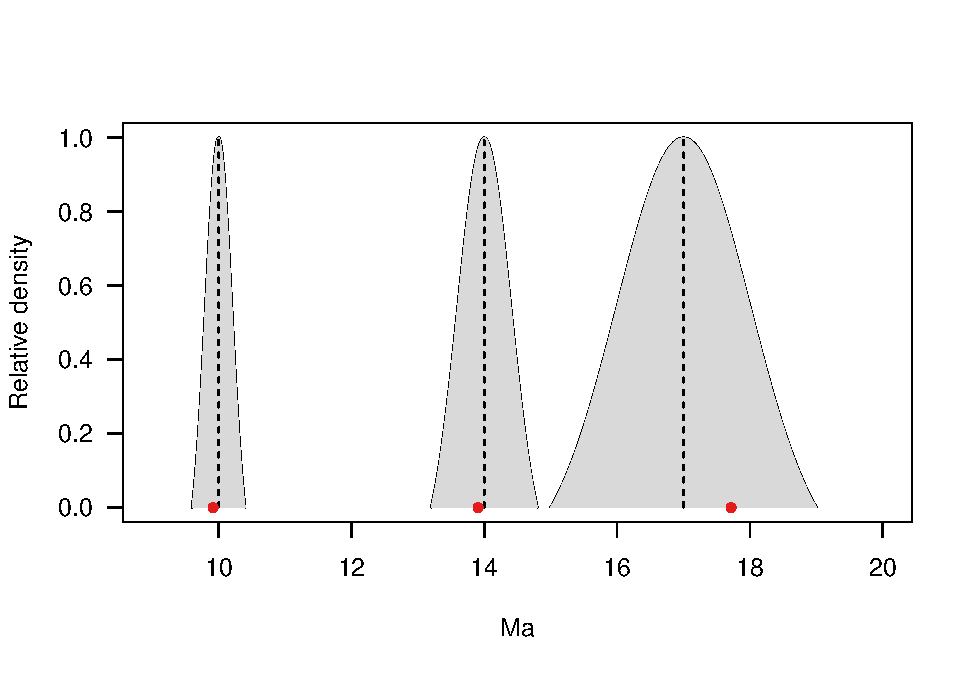
\includegraphics[width=120mm]{figs/ZirconAge.pdf}
\caption{Example of three zircons with measured ages of 10, 14, and 17 Ma ($\mu$; indicated by the dashed vertical lines and black triangles) and standard deviations ($\sigma + \epsilon$; shown by the gray shaded areas). The sampled true ages of the zircons are indicated by the red circles. }
\label{f_zir_age}
\end{figure}


The value of $x_j$, the age of the $j^{\text{th}}$ sample, is determined by two latent variables ($r_j$ and $\mathbf{I}^j$) and constrained by the sampled values of $\mathbf{z}$ such that $x_{i} > x_{i - 1}$ for $i \in \{2, \dots, S\}$.
Specifically, we define as 
\begin{equation}
\zeta_j = \min(\mathbf{z}^{s}), \text{ for } s \in \{j, \dots, S\},
\end{equation}
the minimum age across all zircons included in sample $j$ and in all older samples. 
Thus, $\zeta_j$ represents the upper (older) boundary for the age of sample $j$, which must be younger than all following samples (ordered by depth) and than its youngest zircon.
Under this notation we define the age of a sample as: 
\begin{equation}
x_j = \left\{
\begin{array}{@{}ll@{}}
    r_j (\zeta_j), & \text{if}\ j = 1 \\
    x_{j - 1} + r_j (\zeta_j - x_{j - 1}), & \text{if}\ j > 1 \\
\end{array}\right.
\label{x_constraint}
\end{equation}
where $r_j \in (0, 1)$ is an estimated sample-specific latent parameter determining how close $x_{j}$ is to its lower boundary $x_{j - 1}$ (or to 0 if $j = 1$). 
Thus, when $r_j \approx 0$ the age of the sample is close to its younger boundary and when $r_j \approx 1$ the age of the sample is close to its older boundary. 
%
We also account for the fact that a zircon can be younger than the sample it was found in, for instance due to a dating error or a later recrystallization of the zircon. 
To account for this possibility, we additionally estimate a vector of identifiers $\mathbf{I} = \{I_1, \dots, I_N\}$ that define which zircons (identified by $I = 1$) are older than the sample and therefore used to determine  its upper age boundary  and which zircons (identified by $I = 0$) are younger than the age of the sample. 
Thus, the upper boundary of a sample age is:
\begin{equation}
\zeta_j = \min(\mathbf{z}^{s} \backslash \mathbf{I}^s_0), \text{ for } s \in \{j, \dots, N \}, 
\end{equation}
where $\mathbf{z}^{s} \backslash \mathbf{I}^s_0$ indicates the subset of zircons in sample $s$ with indicator equal to 1. 

We can now define the prior probability of $z_i^j$, i.e. the $i^{\text{th}}$ zircon in sample $j$ as a function of the age of the sample ($x_j$) and an estimated scale parameter $s_j$. 
Specifically we model the prior distribution of zircons in a sample using a compound-Uniform-Cauchy distribution, defined as:
\begin{equation}
P(z_{i,j} | x_j, s_j) = \left\{
\begin{array}{@{}ll@{}}
    z_{i,j} \sim \mathcal{U}(0, 2x_j), & \text{if}\      z_{i,j} < x_j \\
    z_{i,j} \sim \mathcal{C}(x_j, s_j), & \text{if}\      z_{i,j} \geq x_j \\
\end{array}\right.
\end{equation}
where $s_j$ is the sample-specific scale parameter of the Cauchy distribution. 
Under this parameterization, the age of the zircons identified as younger than the sample will have a prior uniform probability ranging from 0 to the age of the sample and rescaled to integrate to 0.5.
The other zircons will instead follow a half-Cauchy distribution with mode equal to the age of the sample (Fig. \ref{f_sample_prob}). 

\begin{figure}[h!]
\centering
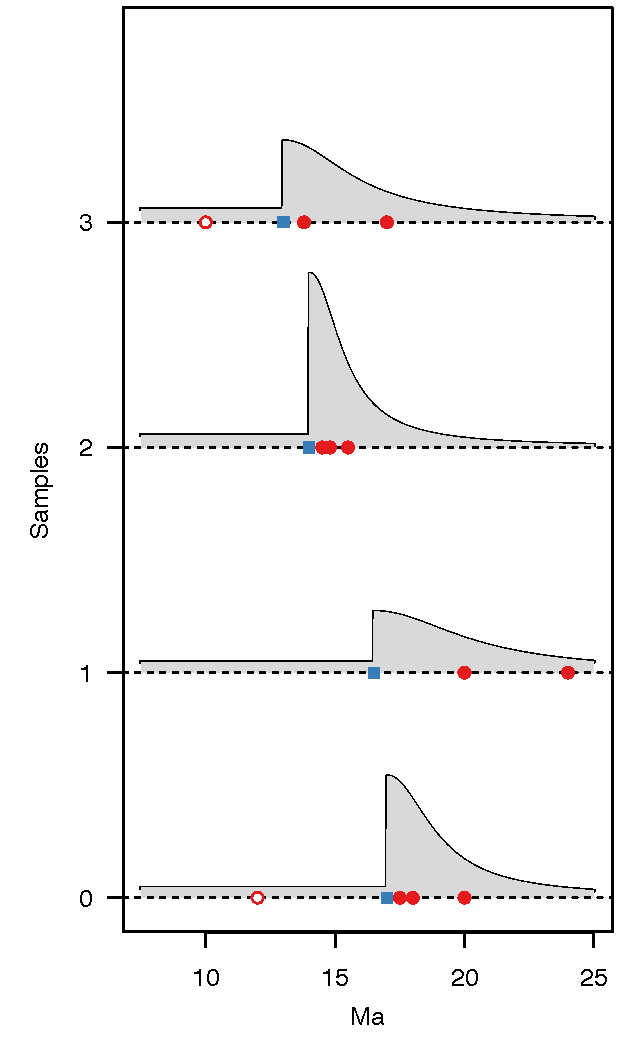
\includegraphics[width=100mm]{figs/SampleProb.pdf}
\caption{Probability distributions of zircon ages in four samples sorted from oldest (sample 0) to most recent (sample 3). Red filled circles indicate zircons  identified as older that the age of the sample, shown as a blue square. Red empty circles indicate zircons identified as younger than the sample. The gray shaded areas display the relative probability distribution of the zircon ages multiplied by the probability of the respective indicator (here set to $P(I = 0) = 0.1$). We note that the maximum age of sample 1 ($x_1$) is not determined by its youngest zircon (of age 20 Ma), but by the age of the previous sample $x_0$. }
\label{f_sample_prob}
\end{figure}

\clearpage
\newpage
\subsubsection{Priors and hyper-priors}
We use a half-Cauchy prior for the vector of scale parameters of the compound Uniform-Cauchy distributions $\{s_1, \dots, s_S \} \sim \mathcal{C}^+(0, \beta)$, where the scale parameter $\beta$ is assumed to be unknown and estimated through MCMC, with a gamma hyper-prior $\beta \sim \Gamma(10, 0.5)$. 
%a normal prior centered on 0 on the vector of bias parameters $\{\eta_1, \dots, \eta_M \} \sim \mathcal{N}(0, 5)$ 
We set an exponential prior on the vector of parameters $\{\epsilon_1, \dots, \epsilon_M \} \sim \text{Exp}(0.1)$.
We use a beta distribution as prior on the vector of parameters $\{r_1 \dots, r_S\} \sim \mathcal{B}(a, b)$ and consider the shape parameters $a$ and $b$ themselves as unknown parameters and assign them exponential hyper-priors, $a, b \sim \text{Exp}(0.1)$.
Finally we use a Bernoulli distribution as prior on the indicators $\{I_1, \dots, I_N\}$ with parameter $p = 0.99$, thus assigning a 0.01 prior probability for a zircon to be younger than the sample it is assigned to. This informative prior assumes that only a small fraction of the zircons might have re-crystallized or is otherwise erroneously dated. 

\subsubsection{Parameter estimation}
The model includes $2N + 2M + 2S + 3$ parameters ($z$ and $I$, $\epsilon$, $s$ and $r$, $a$ and $b$ and $\beta$, respectively). 
All parameters are estimated through Metropolis-Hastings Markov chain Monte Carlo (MCMC). We use a sliding window proposal with reflection at the boundaries for $r$, normal kernel proposals for $z$, binomial proposals for $I$. We use multiplier proposals on all other parameters since they only span the positive range. 


\subsubsection{Adding a maximum age constraint}
A maximum age constraint can be added to the age model by including an additional sample with a single age measures with no dating error. This artificial sample will therefore include a single measured age of fixed age $\mu^{S+1}$ and standard deviation $\sigma^{S+1} = 0$ to enforce a hard boundary. 
This artificial sample is assigned a fixed indicator $I^{S+1} = 1$ and its true age is set equal to the measured one $x^{S+1} = \mu^{S+1}$. 
This approach enforces a maximum age constraint to the estimated ages of all following samples. 

\begin{equation}
x_j = \left\{
\begin{array}{@{}ll@{}}
    r_j (\zeta_j), & \text{if}\ j = 1 \\
    x_{j - 1} + r_j (\zeta_j - x_{j - 1}), & \text{if}\ j > 1 \\
\end{array}\right.
\end{equation}



\clearpage
\subsection{Results}
The preliminary results obtained under this model are shown in Table \ref{table_res}. 


%%%%%%
\renewcommand\baselinestretch{1.2}\selectfont
\begin{longtable}{llll}
\caption{Estimated ages from preliminary MCMC analyses (5 replicates). }\\
\hline
Sample name  &  \multicolumn{3}{l}{Estimated ages (Ma)} \\ 
   &  mean  &  median  &  95\% HPD interval \\ 
\hline
JG-R88-4  &  10.166  &  10.1492  &  9.1341 -- 11.599 \\ 
Z6  &  11.044  &  11.1778  &  9.6965 -- 12.083 \\ 
TVV-01  &  11.069  &  11.207  &  9.7002 -- 12.104 \\ 
JG-R88-2  &  11.0701  &  11.207  &  9.6982 -- 12.104 \\ 
Z5  &  11.078  &  11.2138  &  9.635 -- 12.108 \\ 
004  &  11.518  &  11.567  &  10.718 -- 12.369 \\ 
002  &  11.543  &  11.593  &  10.719 -- 12.351 \\ 
003  &  11.566  &  11.616  &  10.758 -- 12.372 \\ 
LV13  &  11.603  &  11.646  &  10.769 -- 12.390 \\ 
KS4  &  11.678  &  11.720  &  10.834 -- 12.420 \\ 
LV8  &  11.777  &  11.830  &  10.936 -- 12.441 \\ 
Z4  &  11.928  &  11.975  &  11.191 -- 12.509 \\ 
JG-R89-2  &  12.052  &  12.087  &  11.458 -- 12.600 \\ 
SEL-02  &  12.070  &  12.102  &  11.433 -- 12.633 \\ 
TVV-04  &  12.074  &  12.103  &  11.433 -- 12.663 \\ 
Z3  &  12.077  &  12.103  &  11.433 -- 12.700 \\ 
JG-R90-1  &  12.171  &  12.191  &  11.538 -- 12.805 \\ 
Z2  &  12.179  &  12.197  &  11.472 -- 12.778 \\ 
JG-R89-3  &  13.082  &  13.115  &  12.657 -- 13.471 \\ 
JG-R90-3  &  13.093  &  13.124  &  12.657 -- 13.466 \\ 
44011  &  13.095  &  13.125  &  12.657 -- 13.466 \\ 
JG-R89-1  &  13.096  &  13.127  &  12.657 -- 13.469 \\ 
UR-02  &  13.096  &  13.127  &  12.657 -- 13.472 \\ 
UR-01  &  13.229  &  13.241  &  12.700 -- 13.761 \\ 
Z1  &  15.097  &  14.769  &  12.207 -- 17.879 \\ 
44017  &  19.521  &  17.700  &  16.513 -- 26.267 \\
\hline
\label{table_res}	
\end{longtable}
\renewcommand\baselinestretch{1.66}\selectfont
%%%%%%




\end{document}




























